\section{Выигрыш игрока Студент}

\quad Теперь на квадрате $(\mu, \lambda) \in [0, 1]^2$ мы рассмотрели
все точки и для каждой нашли оптимальные пары 
$\big(p^*(\mu, \lambda), q^*(\mu, \lambda)\big)$.
Теперь для всех возможых пар из квадрата
$(\mu, \lambda) \in [0, 1]^2$ в соответсвующих
оптимальных парах найдём значения функции:
$$
	\overline G(p^*(\mu, \lambda), q^*(\mu, \lambda), \mu)=
	p \min \Big\{
		\dfrac{q}{\mu};
		\dfrac{1-q}{2(1-\mu)}
	\Big\} + (1 - p) \min \Big\{
		\dfrac{q}{2\mu};
		\dfrac{1 - q}{1 - \mu}
	\Big\}
$$

Получим следующую систему в зависимости от значений  $\mu$ и $\lambda$:

$\overline G(p, q, \mu) =
\begin{cases}
	\dfrac{1}{2}, & 
	\mu = \{0,1\}, \, \lambda \in [0, 1) 
	\\
	[\frac{1}{2}, 1], & 
	\mu = 0, \, \lambda = 1 \cup 
	\mu = 1, \, \lambda = 0
	\\
	\dfrac{1}{2-\mu}, &	
	\mu \in (0, 1), \, \lambda \in 
	(0, 2\dfrac{1 - \mu}{2 - \mu})
	\\
	\dfrac{1}{1 + \mu}, & 
	\mu \in (0, 1), \, \lambda \in 
	(\dfrac{1 - \mu}{1 + \mu}, 1]
	\\
	\Big[
		\dfrac{1}{2}, \, \dfrac{1}{2-\mu}
	\Big], &
	\mu \in (0, 1), \lambda \in 2\dfrac{1 - \mu}{2 - \mu}
	\\ 
	\Big[
		\dfrac{1}{2}, \, \dfrac{1}{1+\mu}
	\Big], &
	\mu \in (0,1), \lambda = \dfrac{1-\mu}{1+\mu}
\end{cases}
$

Изобразим графически множество значений выигрыша в оптимальных точках.
Для этого на квадрате $[0, 1]^{2}$ изобразим все точки, которые 
принимает вектор 
$(\mu \overline G(p^*,q^*,\mu), (1-\mu) \overline G(p^*,q^*,\mu))$ 
при $(\mu, \lambda) \in [0, 1]^2$.

\begin{center}
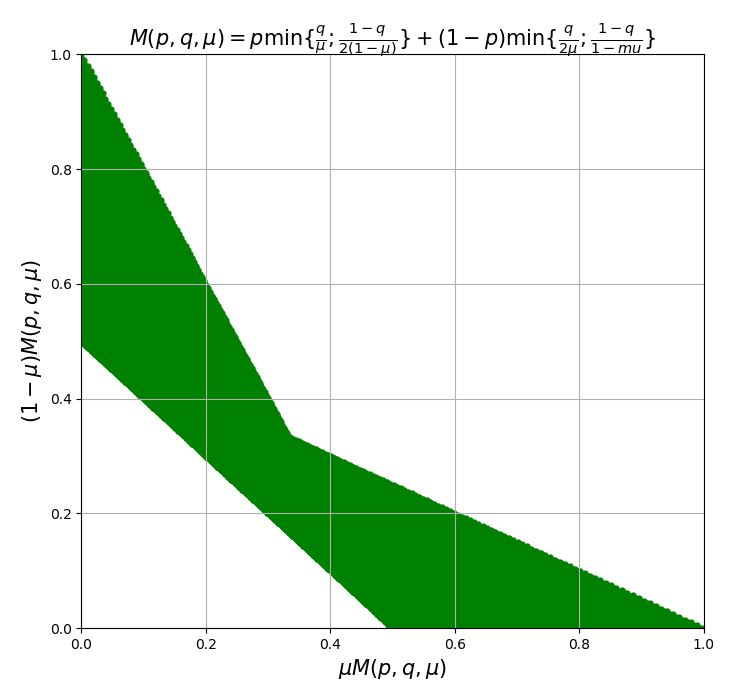
\includegraphics[scale=0.7]{part_2/graf_4}
\end{center}

Поясним график: \\
нижняя огибающая в координатах $X,Y$: $y=\dfrac{1}{2}-x$, \\
верхняя огибающая в координатах $X,Y$: 
$y=
\begin{cases}
	1 - 2x, & x \in [0, \dfrac{1}{3}) \\
	\dfrac{1 - x}{2}, & x \in [\dfrac{1}{3}, 1]
\end{cases}.
$